% This must be in the first 5 lines to tell arXiv to use pdfLaTeX, which is strongly recommended.
\pdfoutput=1
% In particular, the hyperref package requires pdfLaTeX in order to break URLs across lines.

\documentclass[10pt]{article}

% Change "review" to "final" to generate the final (sometimes called camera-ready) version.
% Change to "preprint" to generate a non-anonymous version with page numbers.
\usepackage[final]{acl}

% Standard package includes
\usepackage{times}
\usepackage{latexsym}

% For proper rendering and hyphenation of words containing Latin characters (including in bib files)
\usepackage[T1]{fontenc}
% For Vietnamese characters
% \usepackage[T5]{fontenc}
% See https://www.latex-project.org/help/documentation/encguide.pdf for other character sets

% This assumes your files are encoded as UTF8
\usepackage[utf8]{inputenc}

% This is not strictly necessary, and may be commented out,
% but it will improve the layout of the manuscript,
% and will typically save some space.
\usepackage{microtype}

% This is also not strictly necessary, and may be commented out.
% However, it will improve the aesthetics of text in
% the typewriter font.
\usepackage{inconsolata}
\usepackage{graphicx}

\graphicspath{{./figures/}}

% If the title and author information does not fit in the area allocated, uncomment the following
%
%\setlength\titlebox{<dim>}
%
% and set <dim> to something 5cm or larger.

\title{Using GPT to Predict Company Layoffs}

% Author information can be set in various styles:
% For several authors from the same institution:
% \author{ Alex Straub \and Michael Suehle \and Addison Waller\\}
\author{Michael Suehle \\
  University of Maryland, \\
  College Park \\
 \\\And
  Alex Straub \\
  University of Maryland, \\
  College Park \\
  \\\And
  Addison Waller\\
  University of Maryland, \\
  College Park\\}

% if the names do not fit well on one line use
%         Author 1 \\ {\bf Author 2} \\ ... \\ {\bf Author n} \\
% For authors from different institutions:
% \author{Author 1 \\ Address line \\  ... \\ Address line
%         \And  ... \And
%         Author n \\ Address line \\ ... \\ Address line}
% To start a separate ``row'' of authors use \AND, as in
% \author{Author 1 \\ Address line \\  ... \\ Address line
%         \AND
%         Author 2 \\ Address line \\ ... \\ Address line \And
%         Author 3 \\ Address line \\ ... \\ Address line}

% \author{Michael Suehle \\
%   Affiliation / Address line 1 \\
%   Affiliation / Address line 2 \\
%   Affiliation / Address line 3 \\
%   \texttt{email@domain} \\\And
%   Second Author \\
%   Affiliation / Address line 1 \\
%   Affiliation / Address line 2 \\
%   Affiliation / Address line 3 \\
%   \texttt{email@domain} \\}

\begin{document}
\maketitle

% Abstract
\begin{abstract}
	The technology job market has changed drastically over the last few 
  years with major companies doing multiple layoffs without warning. 
  As this trend continues we wanted to know if there is a way to
   predict these layoffs using alternate data, for example stock 
   market data. To do this we have created a modeling framework 
   utilizing transfer and ensemble learning that takes in past stock 
   data about a company and is able to predict if a layoff has 
   occurred or not. Further, we attempt to use time-series prediction 
   to create future stock data to feed our model for future layoff 
   predictions. We provide a framework that can be extended and 
   modified to adapt to more diverse data and more advanced time 
   series prediction. Utilizing this model, people will be able gain 
   insight into how stock price relates to layoffs, and it opens the
    gate for more sophisticated models to be created to extract more 
    accuracy for percentages and times of layoffs. 
\end{abstract}

%%%%%%%%%%%%%%%%%%%%%%%%%%%%%%%%%%%%%%%%%%%%%%%%%%%%%%%%
%
% Introduction
% 
%%%%%%%%%%%%%%%%%%%%%%%%%%%%%%%%%%%%%%%%%%%%%%%%%%%%%%%%

\section{Introduction}
Over the past couple years the technology sector has experienced a 
large number of mass layoffs. While the exact reason for this 
phenomenon is unclear, we wanted to see if there is a way to predict 
when the next big layoff for a company is coming. To do this we 
created a modeling framework that is able to predict if a company 
will have a layoff in a set time period. Due to time constraints, we 
revised our objective to be a classification problem: can we predict 
whether or not a layoff occurs during a three month period based on 
the stock data? Additionally, can forecasted stock prices help predict 
whether or not a layoff occurs? We decided to pursue these questions 
with domain adaptation and ensemble learning. First, By utilizing 
historical stock and layoff data, we assess if we can use time-series 
prediction and multi layer neural networks to predict whether or not a 
company will layoff people in a 90 day time frame. We test our 
framework with stock data from known periods with and without layoffs, 
and with artificially forecasted periods from our time-series 
forcasting. 

%%%%%%%%%%%%%%%%%%%%%%%%%%%%%%%%%%%%%%%%%%%%%%%%%%%%%%%%
%
% Related Work
% 
%%%%%%%%%%%%%%%%%%%%%%%%%%%%%%%%%%%%%%%%%%%%%%%%%%%%%%%%

\section{Related Work}

\subsection{Layoff Prediction}
We were only able to identify one paper that attempts to predict layoffs 
using machine learning. Prakash and Sakthivel use lasso regression 
to forecast layoffs \cite{predicting-layoffs}. They do not provide the model nor results of the 
model's performance, but they do provide some graphs produced from 
exploratory analysis of the layoff data. Because of this, we could not 
use this as a baseline to compare against. 

\subsection{Incorporating Additional Data for Stock Market Forecasting}
There has been some work on incorporating different types of data to 
improve stock market forecasting.  
Liao et al. incorporate company sentiment data from the news \cite{sentiment-analysis-in-stocks} and 
Ayyappa and Kumar incorporate political data in 
addition to news data to improve stock market forecasting \cite{stocks-news-politics-for-stocks}. 
These studies inspired us to seek sentiment data to use for stock 
market prediction, however we were unable to find a suitable datasource 
in time for this report. 

\subsection{Domain Adaptation for Time Series Data}
As a result of our inability to find suitable data, we looked to use 
domain adaptation to improve stock market predictions. We identified 
three different potential domain adaptation methods for time series 
data. Jin et al. attempt to do domain 
adaptation through attention sharing \cite{domain-adaptation-attention-sharing}. \cite{domain-adaptation-structure-alignment} 
attempt to do domain adaptation with causal structure alignment 
between target and source data that occurs at the same time. 
He et al's method, RAINCOAT, attempts to do domain adaptation 
by training an encoder to extract frequency and time features from 
the source and target data and finally training a classifier on those 
features \cite{raincoat}. We decided to use RAINCOAT because it can be applied to our 
problem, it achieves high performance, and its code is publicly 
available.

\subsection{Data Transform Bagging}
We also experiment with data transform bagging. Data transform bagging
is an alternate version of traditional bagging where each model in the 
ensemble is trained on a different transformation of the same data 
whereas in traditional bagging, each model is trained on different 
samples of the same data \cite{data-transform-bagging}. 


%%%%%%%%%%%%%%%%%%%%%%%%%%%%%%%%%%%%%%%%%%%%%%%%%%%%%%%%
%
% Method
% 
%%%%%%%%%%%%%%%%%%%%%%%%%%%%%%%%%%%%%%%%%%%%%%%%%%%%%%%%

\section{Methods}

Our original objective was to create a model that could predict the 
number of layoffs a company would have in a future time-period. To do 
this we attempted to do Domain Adaptation to Transform Stock Data to 
the domain of the layoff data. Then we wanted to input this transformed 
data into a forecasting model to predict the layoffs. As seen in Figure 
\ref{figure:failed_forecast}, the transformer mapped all the stock 
prices to 0. We believe this was unsuccessful due to the sparsity of 
our data. 

\begin{figure}[h]
  \centering
  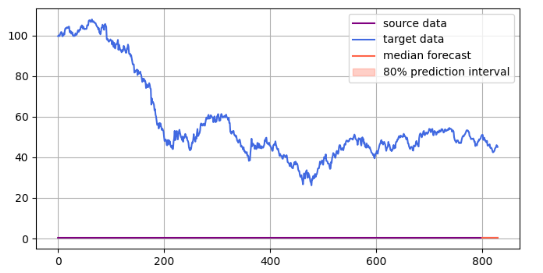
\includegraphics[width=0.5\textwidth]{{/failed_forecast}}
  \caption{Stock data (target data) the transformer was supposed to be 
  able to predict compared to the actual data the transformer predicted
   (source data)}
  \label{figure:failed_forecast}
\end{figure}

Due to time constraints, we revised our objective to be a 
classification problem: can we predict whether or not a layoff occurs 
during a three month period based on the stock data? Additionally, can 
forecasted stock prices help predict whether or not a layoff occurs? 
To achieve this new objective we created four different sets of data 
for each company that spanned three months: real stock data that 
contained no layoffs, real stock data that contained layoffs, chronos 
generated stock data with no layoffs, chronos generated stock data 
with layoffs. Chronos is a zero-shot time series data forecaster 
\cite{chronos}. We used the RAINCOAT algorithm to train an encoder to 
extract the features of both the chronos generated data (source data) 
and real stock data (target data) and a classifier to predict whether
a layoff occurs or not based on the extracted features. This is 
visualized in \ref{figure:raincoat-diagram}. For a baseline classifier 
we used the basic binary classifier and trained it on the real stock 
data. The classifiers would produce a 1 or 0 depending on whether 
there was a layoff (1) or not (0). 

\begin{figure}[h]
  \centering
  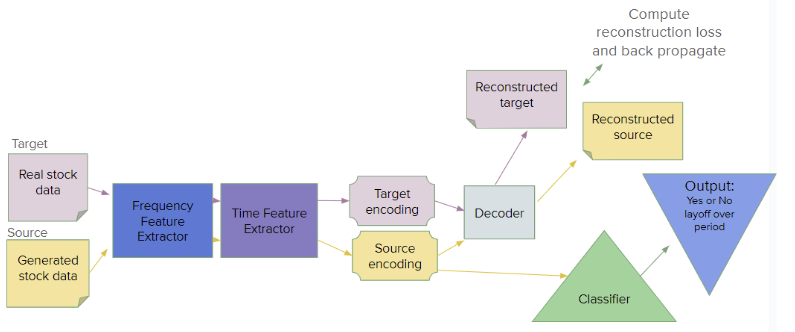
\includegraphics[width=0.5\textwidth]{{/raincoat_diagram}}
  \caption{The architecture of RAINCOAT is as follows. A frequency 
  feature extractor and a time features extractor are trained to
   produce encodings of both the target and source data. Those 
   encodings are decoded and the reconstruction loss is back 
   propagated through the extractors. Simultaneously, a classifier 
   is trained on the encoding of the source data.}
  \label{figure:raincoat-diagram}
\end{figure}

The next classifier we built was an ensemble of three different 
classifiers using a bagging method. Each of these classifiers was 
trained on the real stock data but the data was normalized in 
different ways. The first classifier was trained on z-score 
normalization, the second was trained on proportion to average 
price across periods, and the third was trained on min-max scaling. 
These classifiers then output a probability which represents the 
percentage at which they predict a layoff will happen in the set 
timeframe. We use this probability to create a binary classification, 
where when probability is greater than 0.5, it indicates there is a 
layoff, and less than, no layoff. Each of these classifiers performed 
well, but to further improve performance, we implemented two different 
ensemble strategies. The first was to produce a confidence score by 
taking all the probabilities produced by the classifiers, adding them 
together, and dividing them by three to get an average. If that 
average is over 0.5, then the model predicted there was going to be a 
layoff, if the average is under 0.5 then the model predicted that 
there was not going to be a layoff. The second way to further improve 
performance was to take the binary conversion of the probability 
produced by the classifiers and perform majority voting. For example, 
if two classifiers output a 1 (yes layoff) and the third output a 0 
(no layoff), the overall classifier would predict that there was 
going to be a layoff. The structure can be seen in Figure 
\ref{figure:ensemble-diagram}. Both of these bagging methods perform 
well, results of which will be talked about in later sections of the 
paper.

\begin{figure}[h]
  \centering
  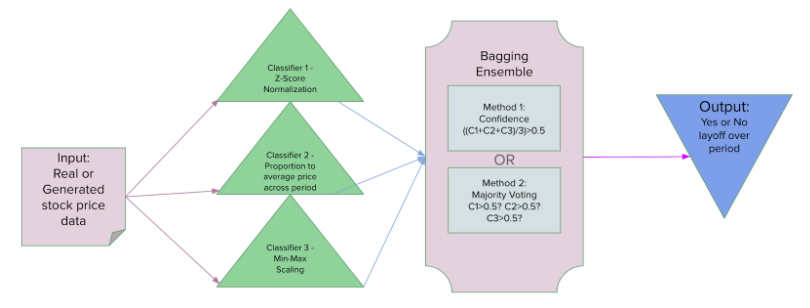
\includegraphics[width=0.5\textwidth]{{/ensemble_diagram}}
  \caption{Flowchart of bagging ensemble classification method}
  \label{figure:ensemble-diagram}
\end{figure}

%%%%%%%%%%%%%%%%%%%%%%%%%%%%%%%%%%%%%%%%%%%%%%%%%%%%%%%%
%
% Experiments
% 
%%%%%%%%%%%%%%%%%%%%%%%%%%%%%%%%%%%%%%%%%%%%%%%%%%%%%%%%

\section{Experiment}
\subsection{Datasets}
For this project we got our layoff data from the dataset: Tech layoffs 
2020 - 2024 from Kaggle \cite{layoff-dataset}. This dataset has the 
number of people laid off, percentage of company laid off, company 
size before and after layoffs, industry, and date of layoff for 1287 
unique companies. It is 1672 rows total. The information in this
dataset we prioritized is: Company name, Number of people laid off, 
Industry, and Date of layoffs. After these columns had been extracted 
the company names were used to compare them to companies that exist 
in the Nasdaq. If they are listed then they are public companies that 
have stock information. Because we wanted to base our layoff 
predictions off stock data it is important that each company we use 
is public. The next step was to collect the stock information for the 
set of companies. Using the \href{https://pypi.org/project/yfinance/}{yfinance} python library we collected each 
company's stock information from 03/10/2020 to 04/18/2024 which 
consisted of open, high, low, close, and volume. All of these data 
points will allow us to begin to predict the possibility of a company 
layoff. 
\\
We used chronos to generate our forecasted stock market data. For 
every layoff date in the Tech layoffs 2020-2024 dataset, we took a 
window of stocks one year before 45 days before the date and generated 
90 days of forecasted stocks after the year of data. For our stock 
data to be labeled “no layoffs”, we programmatically found 90 day 
periods of time that did not have layoffs for each company in the 
Tech layoffs 2020-2024 dataset and used yfinance to pull real stocks 
and chronos to generate forecasted stock based on the real stocks 
for a year 45 days before the start date of the period. For layoff 
stock data, we test with 260 real 90-day stock price datasets, and 
matching time period and stock 260 Chronos generated datasets. For 
no-layoffs testing we have 228 datasets for real, and 228 matching 
chronos generated datasets.

\subsection{Evaluation}
\subsubsection{Baseline Classifier and RAINCOAT}
We trained a baseline classifier on the real stock data and evaluated 
it on real stock data. To evaluate how well RAINCOAT adapts the domain 
of the chronos generated data to the real data, we trained another 
classifier using RAINCOAT and evaluated it on real stock data. To get 
a comparison to see if RAINCOAT improves performance using chronos 
generated training data, we trained a baseline classifier on the 
chronos generated data and evaluated it on the real stock data. We 
also wanted to test two more practical scenarios where we train a 
classifier on real data and evaluate it on chronos generated data, 
emulating a method for predicting if a layoff is going to occur in 
the future by using the classifier on projected stock prices, and 
training a classifier on both real and chronos generated data in 
the scenario where there is not enough real data, so generated data 
is used to increase the number of samples.  

\subsubsection{Ensemble Classification}
We evaluate our bagging ensemble classification model across layoff 
and no-layoff stock datasets for both real, and chronos generated 
stock prices. We record each accuracy score for each of the 
classification models, as well as accuracy for both of our bagging 
ensemble methods for both real and chronos data. We also obtain 
'matching' ratios, displaying how often the classifier output for 
the Chronos generated data agrees with the classifier output for 
the matching real stock data.  
\\
For an ablation study on the ensemble, we also test performance 
degradation when leaving one of the three classifiers out in the 
ensemble for our confidence strategy.

%%%%%%%%%%%%%%%%%%%%%%%%%%%%%%%%%%%%%%%%%%%%%%%%%%%%%%%%
%
% Results
% 
%%%%%%%%%%%%%%%%%%%%%%%%%%%%%%%%%%%%%%%%%%%%%%%%%%%%%%%%
\section{Results}
\subsection{RAINCOAT Dokmain Adaptation}
\begin{table}[h]
  \centering
  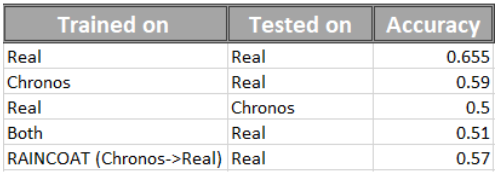
\includegraphics[width=0.5\textwidth]{{/raincoat_results}}
  \caption{Accuracy scores testing the classifiers on generated 
  and real stock data}
  \label{table:raincoat_results}
\end{table}
Table \ref{table:raincoat_results} shows the results of our experiment. 
The baseline model, the classifier trained on real data and tested on 
real data, performed somewhat poorly, achieving an accuracy of 0.65, 
slightly better than random guess of 0.5. The baseline model 
expectedly performed significantly worse on the chronos generated 
data. The classifier trained on chronos generated data and evaluated 
on real data performed worse than the baseline model as expected, 
achieving an accuracy of 0.59. Performance degraded substantially 
when the classifier was trained on both the real and the chronos 
generated data. This is expected since the classifier trained on 
the chronos data performed poorly, but it is surprising that 
performance degraded as much as it did. Finally, the classifier 
trained with the RAINCOAT domain adaptation method performed similarly 
to the classifier trained on chronos data. This implies that the 
RAINCOAT domain adaptation did not improve the performance of the 
classifier.

\subsection{Ensemble Classification (trained on real data)}
\begin{table}[h]
  \centering
  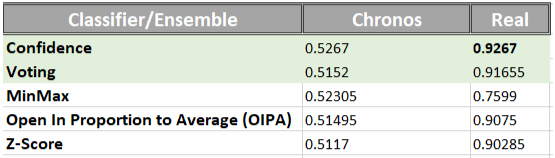
\includegraphics[width=0.5\textwidth]{{/ensemble_results}}
  \caption{Accuracy scores testing the classifier(s) on generated 
  and real stock data}
  \label{table:ensemble_results}
\end{table}
For both layoff and no-layoff stock price periods, we find both the 
individual classifiers and the ensemble bagging output perform 
substantially better when using real stock data compared to the 
Chronos generated data (Table \ref{table:ensemble_results}). On real 
data, we achieve high accuracy in all of the classifiers trained, with 
the Open In Proportion to Average normalization and Z-score 
normalization models leading the individual classifiers. Both 
of our ensemble methods performed better than any of the individual 
classifiers on real data, with >90\% accuracy. The confidence 
ensemble method performed the best at around 93\% accuracy.

\begin{table}[h]
  \centering
  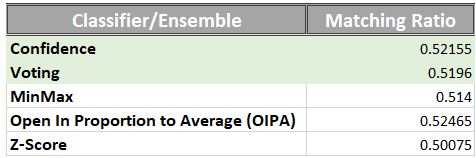
\includegraphics[width=0.5\textwidth]{{/ensemble_match_ratio}}
  \caption{Classification matching ratios by method between Chronos 
  generated and real data}
  \label{table:ensemble_matio_ratio}
\end{table}

We find the matching ratio (the ratio of which the Chronos generated 
data and the matched real data predict the same label when fed into 
the classifier) to be quite poor. Ideally we would see a high
 matching ratio, since that would indicate strong model performance 
 on future-generated Chronos data. Therefore we can not confidently 
 say that we have created a model pipeline to predict future layoffs, 
 since we can not rely on Chronos generated data to be representative 
 of real data. 

 \subsection{Ensemble Ablation}
 \begin{table}[h]
  \centering
  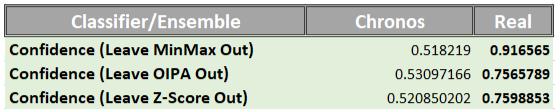
\includegraphics[width=0.5\textwidth]{{/ensemble_ablation}}
  \caption{Accuracy scores testing from leaving one classifier out}
  \label{table:ensemble_ablation}
\end{table}
To bolster our results, we assess the confidence prediction when we 
leave a classifier out of the ensemble. For testing on real data, 
when leaving out MinMax, we see slightly degraded performance when 
compared to the complete ensemble. Omitting either the Z-score 
normalization model or open in proportion to the average model 
yielded significantly degraded performance, of around 18\%. In 
testing on Chronos generated data, we see little or no change in 
confidence prediction, likely due to overall poor model performance
of each of the classifiers in the ensemble for generated data.

%%%%%%%%%%%%%%%%%%%%%%%%%%%%%%%%%%%%%%%%%%%%%%%%%%%%%%%%
%
% Conclusion
% 
%%%%%%%%%%%%%%%%%%%%%%%%%%%%%%%%%%%%%%%%%%%%%%%%%%%%%%%%
\section{Conclusion}
Our results show two main conclusions. The first is that stock data 
generated by chronos is not sufficient for predicting whether or not a
 layoff occurs during the time period the data is generated for. 
 The second is that data transformation bagging greatly improves the 
 performance of the layoff predicting classifier when trained on real 
 data. Although this experiment was not successful at demonstrating 
 viability of forecasted data, it does shed light on a less common 
 version of bagging, transform bagging. Since we achieved high 
 accuracy on our ensemble classifier, it still may be useful for 
 predicting a notion of layoff risk when used with recent stock data, 
 as a positive output could indicate a layoff in the near future.


%%%%%%%%%%%%%%%%%%%%%%%%%%%%%%%%%%%%%%%%%%%%%%%%%%%%%%%%
%
% Future Work
% 
%%%%%%%%%%%%%%%%%%%%%%%%%%%%%%%%%%%%%%%%%%%%%%%%%%%%%%%%
\section{Future Work}
Work progressing from this study can be directed in a number of ways. 
Utilizing more, and different types of data for ensemble classifiers 
to be built upon, such as industry sentiment, company sentiment, 
revenue, and earnings, as well as stock indicators may yield more 
insight into what factors contribute to layoffs. Further, utilizing 
a more advanced, or specified, time-series forecasting model for 
predicting stock price may yield significantly better performance in 
our classification model, enabling the use of the model to predict 
future layoffs. Another area of work is modifying our ensemble 
classification model to predict the percentage of people being laid 
off (vs. company size), enabling the notion of 'severity' in layoff 
prediction. Future work could also include modifying our model 
framework to predict for different time periods, including by week,
or by day predictions. As layoffs continue to happen in the 
tech-sector, more data will become available for models like ours to 
use, allowing for overall better analysis and forecasting of future 
layoff scenarios.

\bibliography{custom}


\end{document}